\documentclass{article}
\usepackage[utf8]{inputenc}
\usepackage{amsmath, amsfonts, amssymb, graphicx, float}
\usepackage{listings}
\usepackage{color}

\setlength{\footskip}{70pt}
\newcommand{\blue}{\textcolor{blue}}
\newcommand{\red}{\textcolor{red}}

%Some code I found for integrating code easily https://stackoverflow.com/questions/3175105/inserting-code-in-this-latex-document-with-indentation

\definecolor{dkgreen}{rgb}{0,0.6,0}
\definecolor{gray}{rgb}{0.5,0.5,0.5}
\definecolor{mauve}{rgb}{0.58,0,0.82}

\lstset{frame=tb,
  language=java,
  aboveskip=3mm,
  belowskip=3mm,
  showstringspaces=false,
  columns=flexible,
  basicstyle={\small\ttfamily},
  numbers=none,
  numberstyle=\tiny\color{gray},
  keywordstyle=\color{blue},
  commentstyle=\color{dkgreen},
  stringstyle=\color{mauve},
  breaklines=true,
  breakatwhitespace=true,
  tabsize=3
}

\title{CTA200 Project - A Giant Pulse of the Crab Pulsar from Raw Voltage Data}
\author{Parasar Thulasiram}
\date{May 19, 2020}

\usepackage{biblatex}
\addbibresource{sample.bib}

\begin{document}

\maketitle

\section{Introduction}
The Crab Pulsar is the peculiar central star of the Crab nebula, the remnant of a supernova in the constellation of Taurus. Its uniqueness lies in radio astronomy, for it is one of the most well known pulsars to emit giant radio pulses, 
highly intense pulses of radio emission that surpass the mean flux density emitted by orders of magnitude \cite{2019MNRAS.490L..12B}.

Due to the rotation of pulsars and the fact that the jet of electromagnetic radiation is on both sides of the star, it is possible for giant pulses (GP)
to be detected twice per pulsar rotation as the GP main pulse (MP) 
or the GP inter pulse (IP). 
However, not all pulsars emit GPs, not all GP pulsars emit only GPs, and not every GP pulsar shows both GP MP
and GP IP. Moreover, a GP is only detectable if the sensitivity of the instrument is fine enough due to their short duration
 \cite{2012hpa..book.....L}.

In order to study the statistical properties of GPs, we must include its profile of emitted frequencies, called the spectral index, and its intensity variations over time, called the amplitude variations \cite{2019MNRAS.490L..12B}. We worked through the raw dataset with the baseband package and explicitly demonstrate how to find the pulse from the raw data for the one-week project.

The data analyzed was baseband voltage data, which was collected by the 10 m telescope at the Algonquin Radio Observatory, located in the Unorganized South Nipissing District in Ontario, Canada. The baseband data contains 2 linear polarizations, 1024 frequency channels from 800 to $\sim 400$ MHz, and a timing resolution of $2.56 \ \mu$s, which is an advantage to study GPs due to their smaller timing window.

Fundamentally, the purpose of this project was to learn how to use the python baseband package\footnote{\url{https://baseband.readthedocs.io/en/stable/}} and to interpret the raw Crab Pulsar baseband data in search of a giant pulse.  

\section{Procedure}
After installing the necessary packages, the first problem was to read a single .vdif file containing raw data. This required passing through the sampling rate of the data collected into the
method vdif.open() as follows
\begin{lstlisting}
from baseband import vdif
fh = vdif.open(file, 'rs', sample_rate = sample_rate)
\end{lstlisting}
where the sampling rate is $\tfrac{400}{1024} \text{ MHz}.$
Following this, the method
\begin{lstlisting}
vdif.info()
\end{lstlisting}
could be used to determine the data collection start time, end time, frequency channel count, and frame count. Those values are 2020-04-23T23:22:49.009187688, 2020-04-23T23:22:49.010211687, 1024, and 65536, respectively.\\
\\
However, the entire raw data set was contained within 21 separate files, meaning that the whole data set needed to be synthesized and then interpreted. This required the use of a function called 'sequentialfile' imported from the baseband.helpers module. This function turns a list of files of the same file format into a single contiguous file that can then be opened identically as above. In full programming detail,
\begin{lstlisting}
from baseband import vdif
from baseband.helpers import sequentialfile as sf
filenames = sorted(glob.glob(filepath))
fraw = sf.open(filenames, 'rb') #contiguous file
fh2 = vdif.open(fraw, 'rs', sample_rate = sample_rate)
\end{lstlisting}
Since it is interpreted as a single file, the .info() method can be used to obtain the same information as above. The start time of the dataset was 2020-04-23T23:22:49.752655360 and the end time was 2020-04-23T23:22:51.514263040.\\
\\
The next step was to de-disperse the raw data so as to obtain a singular, observable peak in the pulse \cite{2012hpa..book.....L}. Essentially, the pulse travels through the Inter-stellar Medium (ISM), which contains free electrons that act as a fluid with some refractive index. This index is frequency dependent and so some frequencies arrive at the observation site sooner than others, as their velocities are dependent upon their respective indices. The signal is thus spread out in time rather than forming a uniform pulse i.e. it is dispersed. An algorithm called coherent de-dispersion was run to remove this dispersion so that the eventual plot would look like a pulse rather than a very skewed distribution. The core equation behind this algorithm is the delay dispersion equation, which gives the arrival time delay between two frequencies \cite{2012hpa..book.....L}:
 \begin{equation*}
     \Delta t = D*\left( \frac{1}{f_1^2} - \frac{1}{f_2^2}\right)*DM,
 \end{equation*}
 where $D \approx 4148.808$  MHz$^{2}$pc$^{-1}$cm$^3$s and $DM$ is the dispersion measure, the integrated column density of free electrons along the line of sight, in pc cm$^{-3}$. The crab pulsar's de-dispersion time was found to be approximately $1.107 s$ from 800 to 400 MHz with DM = 56.7546 pc cm$^{-3}.$ This corresponds to a number of samples of 430027. More details on the de-dispersion algorithm will be discussed in the algorithm section.\\

The de-dispersed raw voltage data was transformed into intensity over time data, which allows for graphing and readability/interpretability. The voltage has two linearly polarized components. These components were added together to form the intensity data in the following way:
\begin{lstlisting}
polx = z_cohdd[:,0,:]
poly = z_cohdd[:,1,:]
Iraw = np.real(polx)**2 + np.imag(polx)**2 + np.real(poly)**2 + np.imag(poly)**2
\end{lstlisting}
where 
\begin{lstlisting}
z_cohdd
\end{lstlisting} is the coherently de-dispersed data and has shape (1024, 2, 195311) after transposition.\\
\\
These data contain noise from miscellaneous extraneous sources. To visualize the plot without being distracted by red-herring intensity data, this noise must be removed, and it was done so with the application of this algorithm.

\begin{lstlisting}
for i in range(1024):
    Iraw[i,:] -= np.nanmedian(Iraw[i,:]) 
    Iraw[i,:] /= np.nanstd(Iraw[i,:])
    Iraw[i,:] -= np.nanmean(Iraw[i,:])
\end{lstlisting}
For each channel, we first subtracted the median to filter out the noise. Then, we divided the standard deviation to normalize the signal. Finally, we subtracted the mean of each frequency, so that the noise baseline would be zero.
\\

\section{Algorithm}
Coherent de-dispersion works by using the observed voltage to derive the voltage just after emission so as to calculate the signal off the true physical effect rather than off the data that was dispersed through the ISM \cite{2012hpa..book.....L}. Fundamentally, the change in signal due to the ISM is modelled by a phase-only filter function $H,$ which can be determined by the observed voltages and their fourier transforms, as well as a relation between the phases given as follows:
\begin{equation*}
    \Delta \Psi = \int\limits_0^d (k_R-k_L) dl,
\end{equation*}
where $k_R$ and $k_L$ are the wave numbers of the right and left circularly polarized waves and $d$ is the distance to the pulsar \cite{2012hpa..book.....L}.
$H$ inverse is applied to the observed voltage's fourier transform to obtain the emitted voltage, which is transformed back into the time domain, as if the observed data is being pulled back to reveal the actual data. This algorithm can be run in real time, with dedicated processors doing the computations. In comparison to another algorithm called incoherent de-dispersion, coherent de-dispersion is less accurate but also less computationally intensive and thus faster, also working with polarization data.\\

The final step was to plot the data in two ways: using a waterfall plot - colour map with frequency on $y$-axis, time on $x$-axis, and intensity as the colour - and using a standard intensity vs time graph. Those plots are shown below with captions.\\

\begin{figure}[h!]
  \centering
  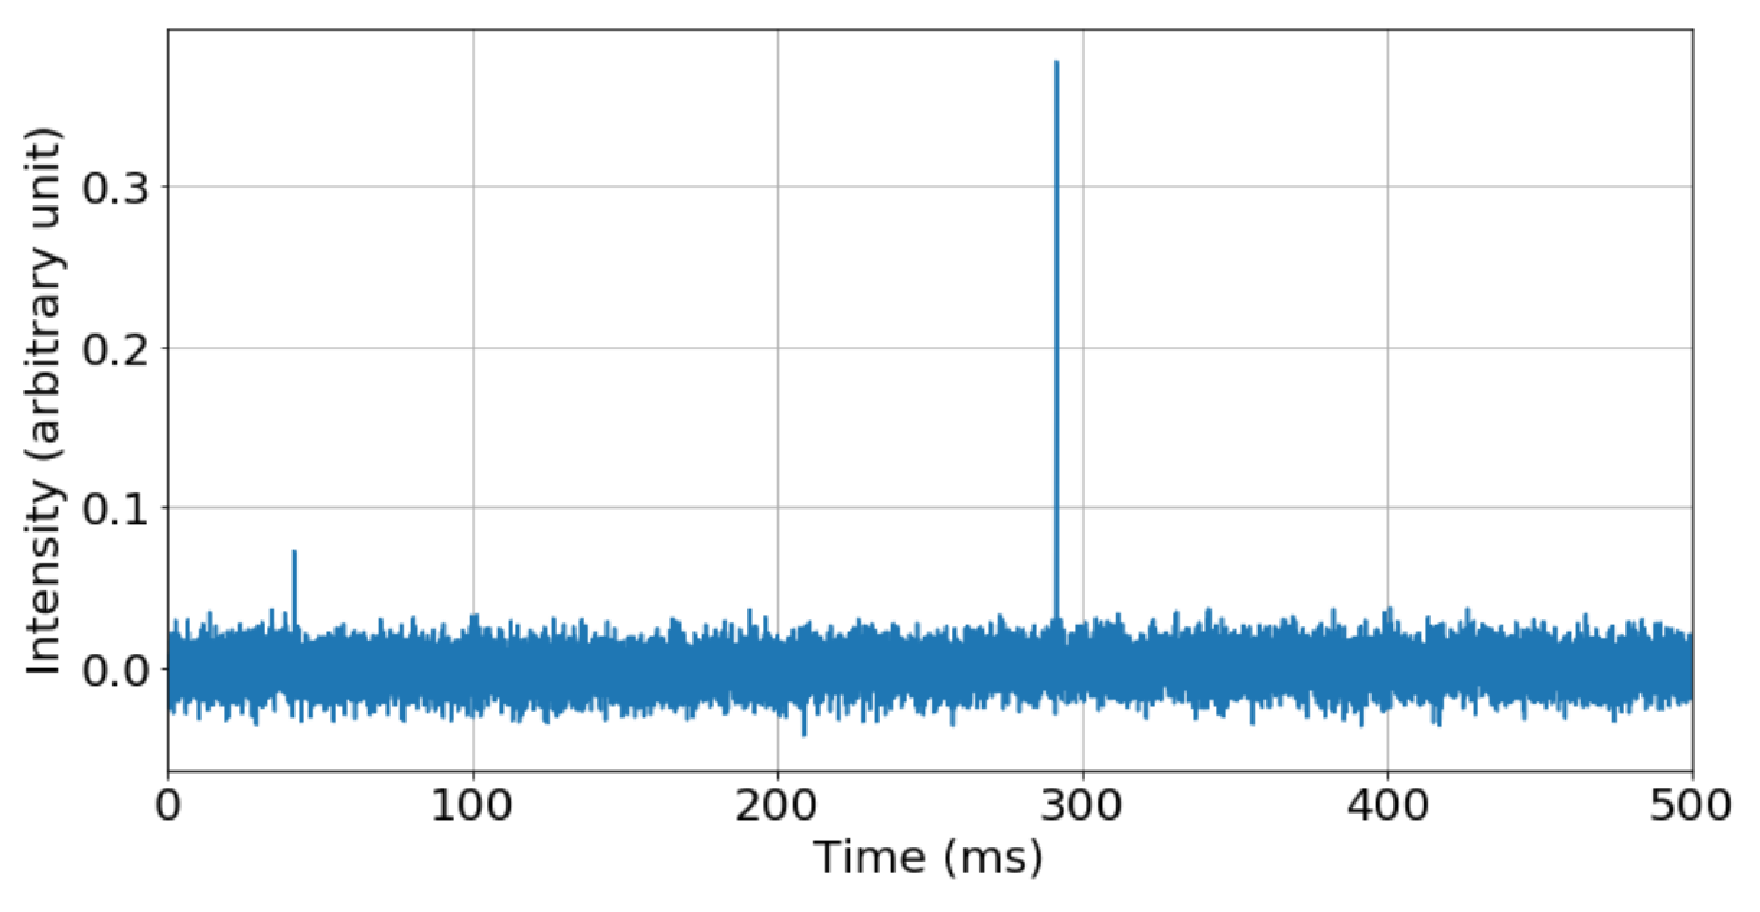
\includegraphics[width=1.0\textwidth]{ts_500ms.pdf}
  \caption{A time-series plot of the coherently de-dispersed, filtered intensity data with a duration of 500 ms. The main peak located at approximately 291.6 ms is a giant pulse.}
\end{figure}
\begin{figure}[H]
  \centering
  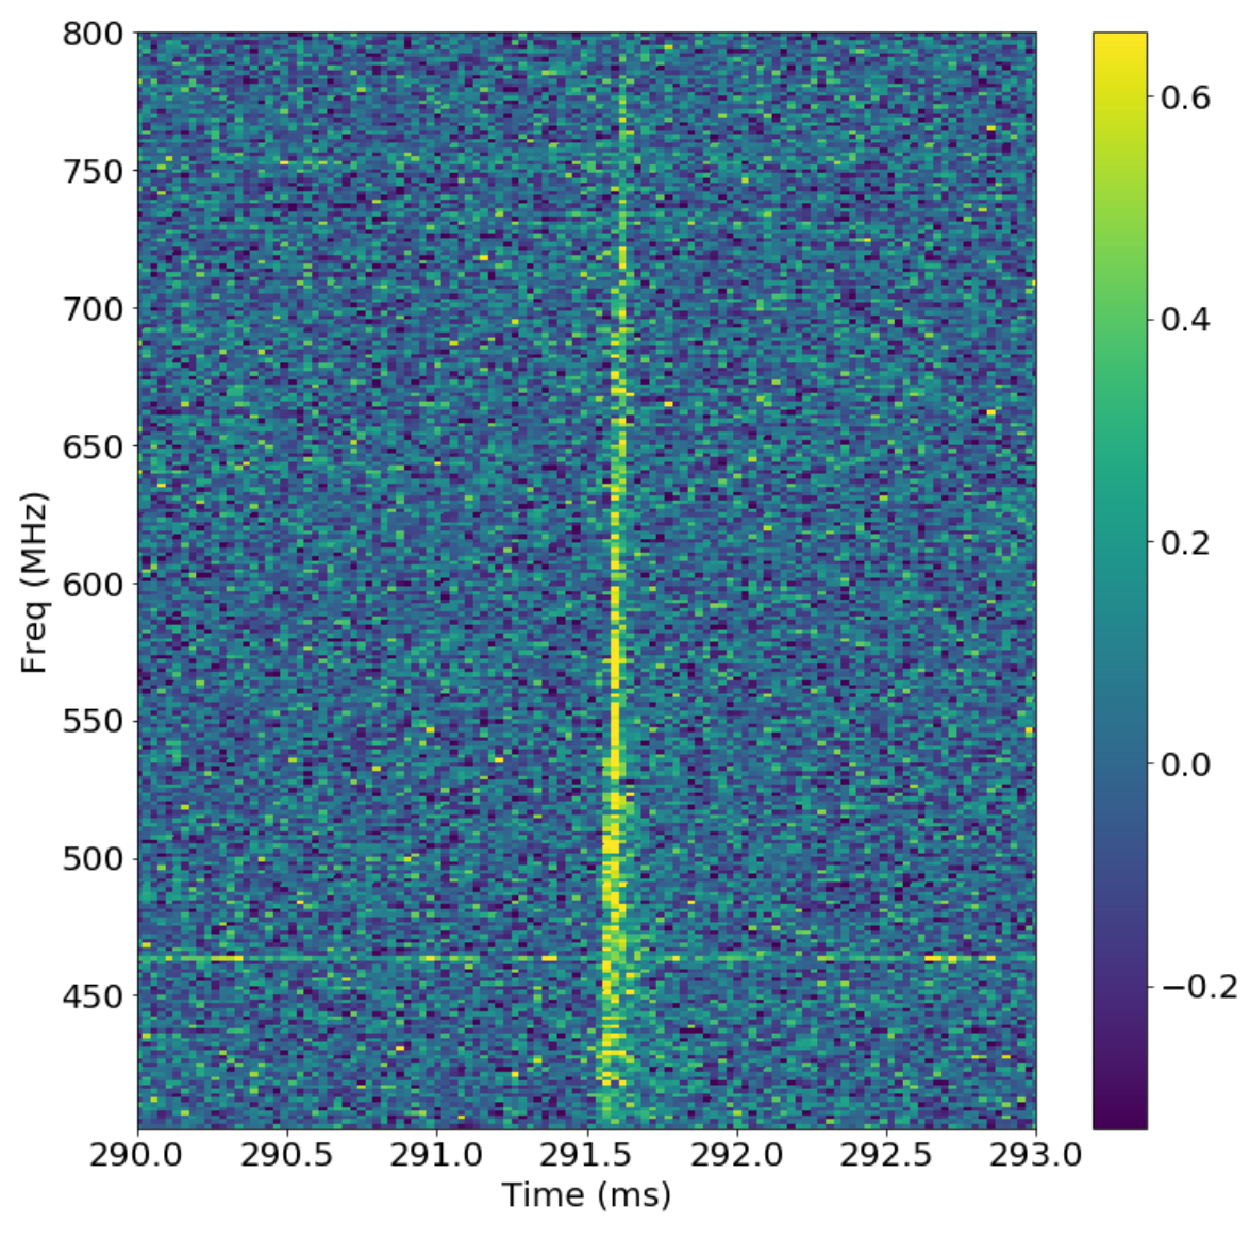
\includegraphics[width=0.9\textwidth]{wf_3ms.pdf}
  \caption{A waterfall plot of the coherently de-dispersed, filtered intensity data with a duration of 3 ms. There are 1.56 MHz per frequency bin and 25.6 $\mu$s per time bin}
\end{figure}
\begin{figure}[H]
  \centering
  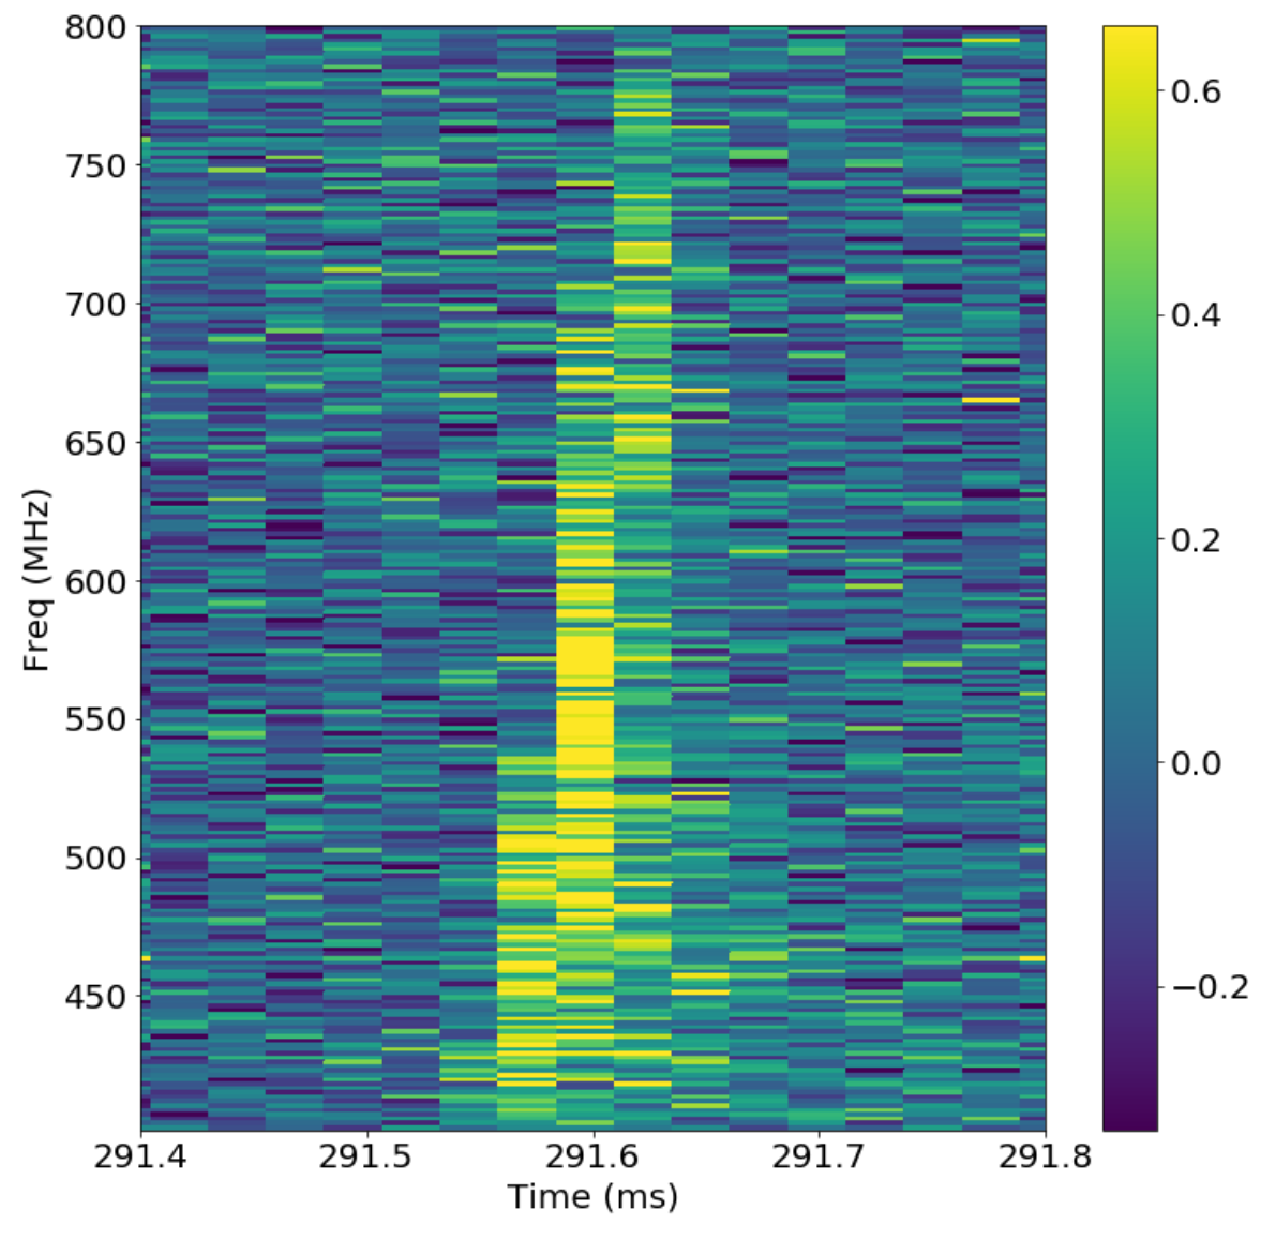
\includegraphics[width=0.9\textwidth]{wf_400mis.pdf}
  \caption{A waterfall plot of the coherently de-dispersed, filtered intensity data with a duration of 0.4 ms. There are 1.56 MHz per frequency bin and 25.6 $\mu$s per time bin.}
\end{figure}

\section{Conclusion}
In conclusion, the analysis successfully detected a clear peak at $\sim 291.6$ ms. This peak is significantly brighter than the peak at $\sim 41$ ms, which is also a giant pulse. We can be certain about this since the sensitivity of the telescope used is low due to its small dish size, meaning that only bright pulses are detectable \cite{2012hpa..book.....L}. Consistent brightness is observable at $\sim 460$ MHz, which could indicate RFI.

\printbibliography

\end{document}
